\documentclass[envcountsect,compress]{beamer}

\mode<presentation>
{
  \usetheme{JuanLesPins}%{Antibes}{Montpellier}
  \setbeamercovered{transparent}
  \usecolortheme{rose}
  \setbeamertemplate{footline}{\hfill\insertframenumber}
  %\beamerdefaultoverlayspecification{<+->}
}

\usepackage[T1]{fontenc}
\usepackage[latin1]{inputenc}

% usual fonts in formulas
\usefonttheme[onlymath]{serif}

% mathfonts and symbols
\usepackage{amssymb,amsmath}

\usepackage{framed}
\usepackage{caption}
\usepackage{subcaption}

% replace some fonts from EC to CM for nice PDF
%\usepackage{aeguill}

% to fix many problems with different symbols
\usepackage{txfonts}

% babel
\usepackage[english]{babel}

% web addresses
\usepackage{url}

\usepackage{caption}
\usepackage{subcaption}
\usepackage{enumerate,graphicx,psfrag}%

\setbeamercovered{transparent=5}%{invisible }%{dynamic}
%\setbeamercolor{normal text}{fg=black,bg=mylightgrey}
%\setbeamercolor{alerted text}{fg=red!80!black}
%\setbeamercolor{postit}{fg=black,bg=yellow}

% Format for theorems and similar.
\theoremstyle{definition}
\setbeamertemplate{theorems}[numbered]
\newtheorem{remark}[theorem]{Remark}
%\newtheorem{defn}[theorem]{Definition}
%\newtheorem{eg}[theorem]{Example}
% \newtheorem{notn}[theorem]{Notation}
% \newtheorem{lemma}[theorem]{Lemma}
% \newtheorem{conj}[theorem]{Conjecture}
% \newtheorem{cor}[theorem]{Corollary}
% \newtheorem{prop}[theorem]{Proposition}
% \newtheorem{res}[theorem]{Result}
\newtheorem{remarks}[theorem]{Remarks}
% \newtheorem{egs}[theorem]{Examples}
% \newtheorem{obs}[theorem]{Observation}
% \newtheorem{ex}[theorem]{Exercise}
% \newtheorem{expl}[theorem]{Explanation}
% \newtheorem{aq}[theorem]{Assignment Question}
% \newtheorem{fact}[theorem]{Fact}
% \newtheorem{prin}[theorem]{Principle}
\numberwithin{equation}{section}
%
\newenvironment{eg}{\begin{example}}{\end{example}}% translate from notes.tex conventions
\newenvironment{defn}{\begin{definition}}{\end{definition}}
%%
\def\notes{{\bf !Take notes!\\}}
\newcommand{\be}{\begin{enumerate}[<+->]}
\newcommand{\ee}{\end{enumerate}}
\newcommand{\bd}{\begin{description}[<+->]}
\newcommand{\ed}{\end{description}}
%\newenvironment{mystepwiseitemize}{\begin{itemize}[<+->]}{\end{itemize}}
\newcommand{\biz}{\begin{itemize}[<+->]}
\newcommand{\eiz}{\end{itemize}}

\newcounter{saveenumi}
\newcommand{\seti}{\setcounter{saveenumi}{\value{enumi}}}
\newcommand{\conti}{\setcounter{enumi}{\value{saveenumi}}}

\resetcounteronoverlays{saveenumi}
\renewcommand{\a}{\alpha }
\renewcommand{\b}{\beta }
\newcommand{\G}{\Gamma }
\newcommand{\g}{\gamma }
\newcommand{\D}{\Delta }
\renewcommand{\d}{\delta }
%\def\vd{\vardelta}
\newcommand{\ep}{\epsilon }
\newcommand{\e}{\varepsilon }
\newcommand{\z}{\zeta }
%\eta
\renewcommand{\th}{\theta }
\newcommand{\T}{\Theta }
\renewcommand{\i}{\iota }
\renewcommand{\k}{\kappa }
\renewcommand{\l}{\lambda }
\renewcommand{\L}{\Lambda }
%\mu
%\nu
%\xi
%omicron
%\pi
\renewcommand{\r}{\rho }
\newcommand{\s}{\sigma }
\renewcommand{\S}{\Sigma }
\renewcommand{\t}{\tau }
\newcommand{\up}{\upsilon }
\newcommand{\U}{\Upsilon }
%\phi
\newcommand{\x}{\chi }
%\psi
\newcommand{\W}{\Omega }
\newcommand{\w}{\omega }
%%%%%%%%%%%%%%%%%%%%%%%%%%%%%%%
%%%%%%%%%%%%%%%%%%%%%%%%%%%%%
\newcommand{\pd}{\partial}
\newcommand{\wht}{\widehat}
%\newcommand{\cC}{{\mathcal C}}
%\newcommand{\cdim}{\texttt{cdim}}
\newcommand{\fC}{{\textswab C}}

\newcommand{\NN}{\mathbb{N}}
\newcommand{\ZZ}{\mathbb{Z}}
\newcommand{\RR}{\mathbb{R}}
\newcommand{\CC}{\mathbb{C}}
\newcommand{\QQ}{\mathbb{Q}}
\newcommand{\PP}{\mathbb{P}}
\newcommand{\KK}{\mathbb{K}}
\newcommand{\EE}{\mathbb{E}}
\newcommand{\FF}{\mathbb{F}}
\newcommand{\NPV}{{\operatorname{NPV}}}
\newcommand{\irr}{{\operatorname{irr}}}
%
\newcommand{\cA}{{\mathcal{A}}}
\newcommand{\cC}{\mathcal{C}}
\newcommand{\cD}{{\mathcal{D}}}
\newcommand{\cF}{{\mathcal{F}}}
\newcommand{\cH}{{\mathcal{H}}}
\newcommand{\cJ}{{\mathcal{J}}}
\newcommand{\cK}{{\mathcal{K}}}
\newcommand{\cO}{\mathcal{O}}
\newcommand{\cP}{{\mathcal{P}}}
\newcommand{\cQ}{{\mathcal{Q}}}
\newcommand{\cR}{{\mathcal{R}}}
\newcommand{\cS}{{\mathcal{S}}}
\newcommand{\cV}{{\mathcal{V}}}
\newcommand{\cW}{{\mathcal{W}}}

\newcommand{\la}{\langle}
\newcommand{\ra}{\rangle}
%%%%%%%%%%%%%%%%%%%%%%%%%%%%%%%%%%%%%%%%%%%%%%%
\title[MAS1243]
{
  MAS1243 \& MAS2243\\
  Application of Mathematical methods to Finance
}

\author{A.~Duncan}

\institute[NCL]
{
  Newcastle University\\
  School of Mathematics and Statistics
}

\date[2012/2013]
{
  Semester 1, 2012/2013
}
%\includeonly{options}
\begin{document}

\begin{frame}
\titlepage
\end{frame}

\begin{frame}
  \frametitle{Outline}
  \tableofcontents[pausesections]
  % You might wish to add the option [pausesections]
\end{frame}
\section{Introduction}

\begin{frame}
  \frametitle{}
Let $G = <X|R>$ be a finitely generated group.
The \emph{subgroup  membership problem}, for  fixed subgroup $K$ of $G$,
is to decide whether or not a given  word $w$ in $\FF(X)$ represents an element of  the subgroup $K$.
The \emph{uniform} subgroup membership problem for $G$ is to decide,
given a finite subset $P=\{w,k_1,\ldots ,k_s\}$ of elements of $\FF(X)$,
for some $s\ge 0$,
whether or not $w$ represents an element of  the subgroup $K$ of $G$
generated by $Y=P\backslash\{w\}$.
The  subgroup membership problem for $K$ in $G$ is said to be
\emph{solvable} if there is an algorithm which, on input $w\in \FF(X)$,
outputs ``yes'' if and only if $w$ does represent an element of $K$.
Similarly, the uniform subgroup membership problem for $G$ is \emph{solvable}
if there exists an algorithm which, on input $P$, outputs ``yes'' if
and only if $w$ represents an element of $K$.
\end{frame}
%%%%%%%%%%%%%%%%%%%%%%%%%%%%%%%%%%%%%
\begin{frame}
  \frametitle{}

If $\cV$ is a class of groups and there exists an algorithm to
solve the uniform membership %(search)
 problem for any element of $\cV$ then
we say that $\cV$ has solvable uniform  %(search)
 membership problem.

\begin{theorem}\label{thm:membership}
Let $F_1$ and $F_2$ be finite rank free groups and let $H_1$ and $H_2$
be finitely generated subgroups of $F_1$ and $F_2$, respectively, such
that $H_1$ is isomorphic to $H_2$. Let $G=F_1 \ast_{H_1=H_2} F_2$.
Let $\cF$ be the class of free products with amalgamation, where
factors are free of finite rank, and the amalgamated subgroups are
finitely generated.
Then
\be
\item\label{it:membership}
$G$ has solvable membership problem,
\item \label{it:uni-membership}
$G$ has solvable uniform  membership problem and
\item\label{it:class-uni-membership}
$\cF$ has solvable uniform  membership problem.
\ee
%Moreover the same conclusions hold for the search versions of each of these
%problems.
\end{theorem}
\end{frame}
%%%%%%%%%%%%%%%%%%%%%%%%%%%%%%%%%%%%%
\begin{frame}
  \frametitle{}
\begin{theorem}\label{thm:howson}
Let $G$ be a group from the class $\cF$ defined in Theorem \ref{thm:membership}.
Then $G$ is Howson. 
\end{theorem}
\end{frame}
%%%%%%%%%%%%%%%%%%%%%%%%%%%%%%%%%%%%%
\begin{frame}
  \frametitle{}
Let $F_1=\FF(x_1,x_2,x_3)$ and $H_1=\la h_1,h_2,h_3\ra$, 

 $h_1= x_1^3$, $h_2=x_2x_3x_2^{-1}$ and
$h_3=x_1x_2x_3$.


and let $F_2=\FF(y_1,y_2,y_3,y_4)$ and
$H_2=\la h_1^\prime, h_2^\prime, h_3^\prime\ra$, 
$h_1^{\prime}=y_2^2$,
$h_2^{\prime}=y_3y_4$ and
$h_3^{\prime}=y_1^2y_3y_1^{-1}y_2$.

$G=F_1\ast_{H_1=H_2} F_2$.

$Z=\{z_1,z_2,z_3\}$
$\phi_1(z_i)=h_i$, $\phi_2(z_i)=h'_i$.

\end{frame}
%%%%%%%%%%%%%%%%%%%%%%%%%%%%%%%%%%%%%
\begin{frame}
  \frametitle{}
Elements 
\begin{align*}
f_1 = &x_2x_3^2x_2^{-1} x_1^4x_3^3x_1^{-2}x_3^{-1}x_2^{-1}x_1^{-1} \\
f_2=&x_3^{-1}x_2^{-1}x_1^{-1}x_2x_3^{-1}x_2^{-1}x_1^{-1}
\end{align*}
have normal forms
\begin{align*}
f_1= & (z_2^{2}z_1) x_1x_3^3x_1(z_1^{-1}z_3^{-1})\in H_1S_1^{(1)}H_1\\
f_2= & f_2=(z_3^{-1}z_2^{-1}) x_1^{-1}\in H_1S_1^{(2)}H_1
\end{align*}

\end{frame}
%%%%%%%%%%%%%%%%%%%%%%%%%%%%%%%%%%%%%
\begin{frame}
  \frametitle{}
Let
\[f_3=x_2x_3^{-1}x_1,\, f_4= x_1^4 x_2 x_3 x_1^{-1} x_2^{-1}
\textrm{ and } f_5=x_1x_2x_3x_2x_3^{-2}x_2^{-1},\]
and let
 $f_1^\prime=y_1^2y_3y_1^{-1}y_2y_3y_4y_1y_2
y_3y_4y_2^2$:
normal form
\[f_1^\prime=z_3z_2 y_1y_2 z_2 z_1.\]
\[ f_2^\prime =y_3y_4y_2^{-1}y_1y_3.\]
normal forms of these elements are
\begin{align*}
f_3 & = x_2x_3^{-1}x_1,\\
f_4 &= h_1h_3 x_1^{-1}x_2^{-1},\\
f_5 &= h_3h_2^{-2}\textrm{ and }\\
f_2^\prime &= h_2^\prime y_2^{-1}y_1y_3.
\end{align*}
\end{frame}
%%%%%%%%%%%%%%%%%%%%%%%%%%%%%%%%%%%%%
\begin{frame}
  \frametitle{}
\begin{figure}
\begin{center}
\psfrag{x1}{$x_1$}
\psfrag{x2}{$x_2$}
\psfrag{x3}{$x_3$}
\psfrag{1}{$1$}
\psfrag{2}{$2$}
\psfrag{3}{$3$}
\psfrag{4}{$4$}
\psfrag{5}{$5$}
\begin{subfigure}[b]{.25\columnwidth}
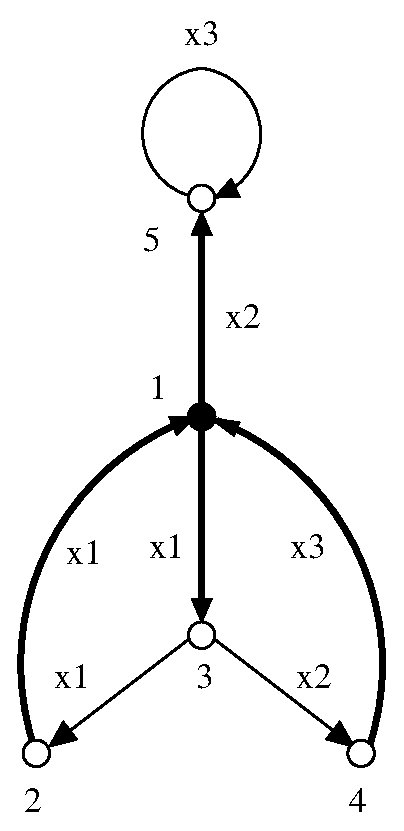
\includegraphics[scale=.4]{../stallh1.eps}
\caption{Stallings automaton $\G_{A_1}$ for $H_1$}
\label{fig:stall1}
\end{subfigure}
\hspace{5mm}
\begin{subfigure}[b]{.25\columnwidth}
\psfrag{a}{$(1,2)$}
\psfrag{b}{$(2,3)$}
\psfrag{c}{$(3,1)$}
\psfrag{d}{$(4,5)$}
\psfrag{e}{$(1,5)$}
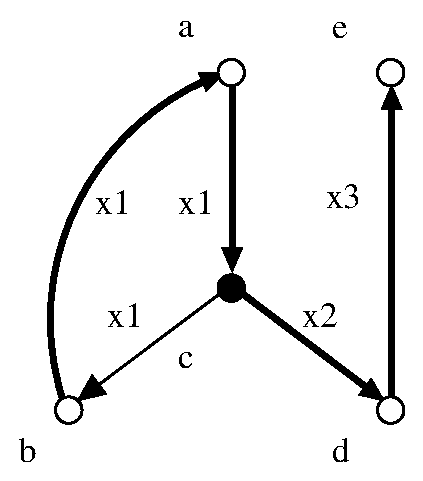
\includegraphics[scale=.4]{../GxG-1.eps}
\caption{$\G_{A_1}\times \G_{A_1}$: connected component of $(3,1)$}
\label{fig:GxG-1}
\end{subfigure}
\hspace{5mm}
\begin{subfigure}[b]{.25\columnwidth}
\psfrag{a}{$(2,1)$}
\psfrag{b}{$(3,2)$}
\psfrag{c}{$(1,3)$}
\psfrag{d}{$(5,4)$}
\psfrag{e}{$(5,1)$}
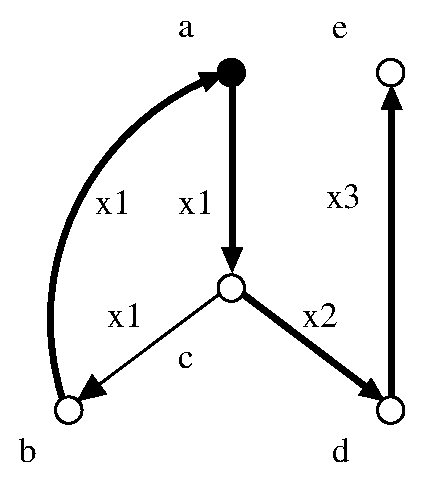
\includegraphics[scale=.4]{../GxG-2.eps}
\caption{$\G_{A_1}\times \G_{A_1}$: connected component of $(2,1)$}
\label{fig:GxG-2}
\end{subfigure}
\end{center}
%\caption{Example \ref{ex:f_1}.}\label{fig:stall}
\end{figure}

\end{frame}
%%%%%%%%%%%%%%%%%%%%%%%%%%%%%%%%%%%%%
\begin{frame}
  \frametitle{}

\end{frame}
%%%%%%%%%%%%%%%%%%%%%%%%%%%%%%%%%%%%%
\begin{frame}
  \frametitle{}

\end{frame}
%%%%%%%%%%%%%%%%%%%%%%%%%%%%%%%%%%%%%
\begin{frame}
  \frametitle{The folded flower automaton of $K$}
%\begin{figure}
~\\[3em]
\begin{center}
\psfrag{a}{$x_1$}
\psfrag{b}{$x_2$}
\psfrag{c}{$x_3$}
\psfrag{r}{$y_1$}
\psfrag{s}{$y_2$}
\psfrag{t}{$y_3$}
\psfrag{x}{$z_1$}
\psfrag{y}{$z_2$}
\psfrag{z}{$z_3$}
\psfrag{u}{$y_4$}
\psfrag{0}{\hspace{-2pt}\raisebox{-2pt}{\scriptsize $0$}}
\psfrag{1}{\hspace{-2pt}\raisebox{-2pt}{\scriptsize $1$}}
\psfrag{2}{\hspace{-2pt}\raisebox{-2pt}{\scriptsize $2$}}
\psfrag{3}{\hspace{-2pt}\raisebox{-2pt}{\scriptsize $3$}}
\psfrag{4}{\hspace{-2pt}\raisebox{-2pt}{\scriptsize $4$}}
\psfrag{5}{\hspace{-2pt}\raisebox{-2pt}{\scriptsize $5$}}
\psfrag{6}{\hspace{-2pt}\raisebox{-2pt}{\scriptsize $6$}}
\psfrag{7}{\hspace{-2pt}\raisebox{-2pt}{\scriptsize $7$}}
\psfrag{8}{\hspace{-2pt}\raisebox{-2pt}{\scriptsize $8$}}
\psfrag{9}{\hspace{-2pt}\raisebox{-2pt}{\scriptsize $9$}}
\psfrag{10}{\hspace{-2pt}\raisebox{-2pt}{\scriptsize $10$}}
\psfrag{11}{\hspace{-2pt}\raisebox{-2pt}{\scriptsize $11$}}
\psfrag{12}{\hspace{-2pt}\raisebox{-2pt}{\scriptsize $12$}}
\psfrag{13}{\hspace{-2pt}\raisebox{-2pt}{\scriptsize $13$}}
\psfrag{14}{\hspace{-2pt}\raisebox{-2pt}{\scriptsize $14$}}
\psfrag{15}{\hspace{-2pt}\raisebox{-2pt}{\scriptsize $15$}}
\psfrag{16}{\hspace{-2pt}\raisebox{-2pt}{\scriptsize $16$}}
\psfrag{17}{\hspace{-2pt}\raisebox{-2pt}{\scriptsize $17$}}
\psfrag{18}{\hspace{-2pt}\raisebox{-2pt}{\scriptsize $18$}}
\psfrag{19}{\hspace{-2pt}\raisebox{-2pt}{\scriptsize $19$}}
\psfrag{20}{\hspace{-2pt}\raisebox{-2pt}{\scriptsize $20$}}
\psfrag{21}{\hspace{-2pt}\raisebox{-2pt}{\scriptsize $21$}}
\psfrag{22}{\hspace{-2pt}\raisebox{-2pt}{\scriptsize $22$}}
\psfrag{23}{\hspace{-2pt}\raisebox{-2pt}{\scriptsize $23$}}
\psfrag{24}{\hspace{-2pt}\raisebox{-2pt}{\scriptsize $24$}}
\psfrag{25}{\hspace{-2pt}\raisebox{-2pt}{\scriptsize $25$}}
\psfrag{26}{\hspace{-2pt}\raisebox{-2pt}{\scriptsize $26$}}
\psfrag{27}{\hspace{-2pt}\raisebox{-2pt}{\scriptsize $27$}}
\psfrag{28}{\hspace{-2pt}\raisebox{-2pt}{\scriptsize $28$}}
\psfrag{29}{\hspace{-2pt}\raisebox{-2pt}{\scriptsize $29$}}
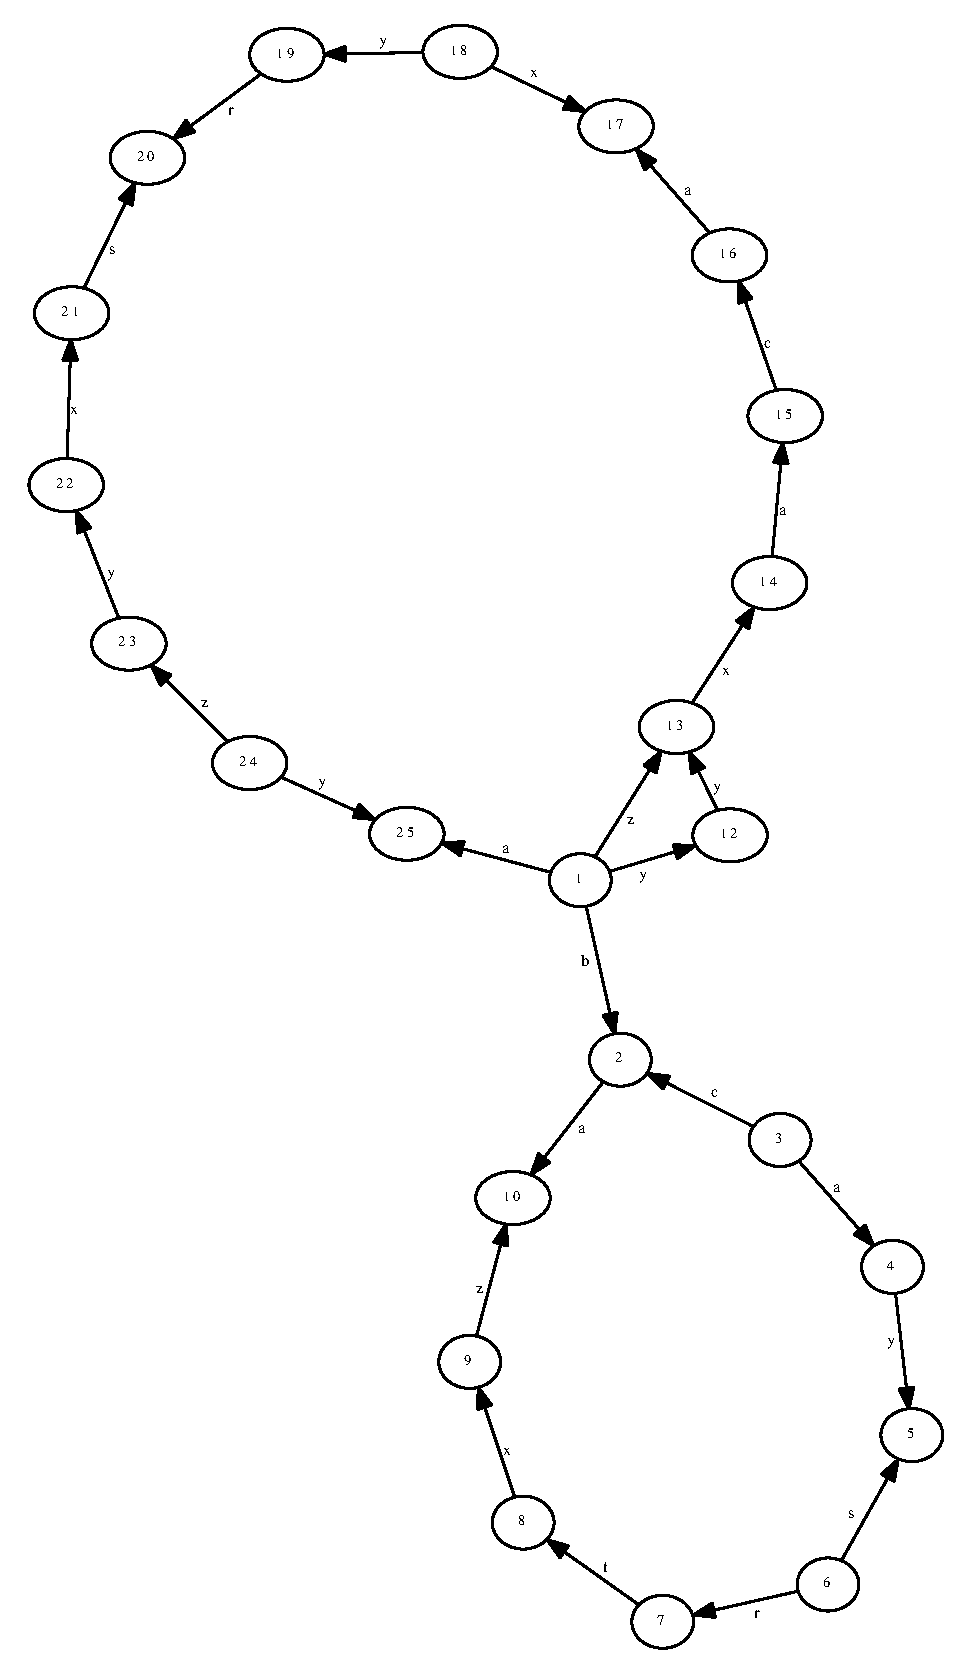
\includegraphics[scale=0.2,bb=0 0 820 720]{../python/ex_K_folded.eps}
%\includegraphics[scale=0.4]{ex_K.eps}
%\caption{The folded flower automaton of $K$}
%\label{fig:Kflower}
\end{center}
%\end{figure}

\end{frame}
%%%%%%%%%%%%%%%%%%%%%%%%%%%%%%%%%%%%%
\begin{frame}
  \frametitle{}

\end{frame}
%%%%%%%%%%%%%%%%%%%%%%%%%%%%%%%%%%%%%
\begin{frame}
  \frametitle{}

\end{frame}
\end{document}



